% ------------------------------------------------------------------------------ %
% The ?rst information LATEX needs to know when processing an input ?le is
% the type of document the author wants to create. This is speci?ed with the
% \documentclass command.
%
%   \documentclass[options]{class}
%
% Here class speci?es the type of document to be created.

\documentclass[a4paper,11pt]{article}

% The above command instructs LATEX to typeset the document as an article with
% a base font size of eleven points, printing on A4 paper.
% ------------------------------------------------------------------------------- %


% ------------------------------------------------------------------------------- %
% While writing your document, you will probably ?nd that there are some
% areas where basic LATEX cannot solve your problem. If you want to include
% graphics, coloured text or source code from a ?le into your document, you
% need to enhance the capabilities of LATEX. Such enhancements are called
% packages. Packages are activated with the
%
%   \usepackage[options]{package}
%
% command, where package is the name of the package and options is a list of
% keywords that trigger special features in the package.
%
% ATTENTION: IN ORDER TO ENABLE THE GREEK TYPESETTING YOU NEED TO INCLUDE IN YOUR
%            PREAMBLE SPECIFIC PACKAGES VIA THE USE OF THE \usepackage COMMAND.
%
%            THE SAME IS TRUE FOR SPECIFIC MATH FONTS ETC.


% * Activating Greek fonts in Latex
  \usepackage[english,greek]{babel} % the last language is the default

  %% > UNCOMMENT if your editor uses iso-8859-7 encoding for Greek (typical in Windows System).
  %\usepackage[iso-8859-7]{inputenc}

  %% > UNCOMMENT if your editor uses Unicode encoding for Greek (typical in POSIX Systems).
  \usepackage[utf8x]{inputenc}

  % One bad thing about the babel package is that it cannot discriminate explicitly between
  % Greek and Latin fonts, so you have to state commands in order to signify where the
  % Latin charecters begin and where they end and the Greek characters begin. For this
  % job the \latintext and \greektext commands exist. However Latex give you the versatility
  % to create wildcards for all of each commands and thus, to create alias with shorter
  % word length. Below we create the aliaces \lt and \gt for the \textlatin and \textgreek
  % commands respectively.

  \newcommand{\lt}{\latintext}
  \newcommand{\gt}{\greektext}


% * Math packages
 % \usepackage{amsthm}
  \usepackage{amsmath}
 % \usepackage{amssymb}

% * graphics package
  \usepackage[pdftex]{graphicx} % remove the 'pdftex' option if not PDFLatex is used.

% * verbatim writing package (mainly used to import program's code)
  \usepackage{verbatim} 
  \setcounter{section}{4}
% ------------------------------------------------------------------------------- %


% ------------------------------------------------------------------------------- %
% Here we set the title, the author and the date of our document.
%
% * Setting the title of the document
  \title{2η Υποχρεωτική Εργασία\\
Στο Μάθημα της Αριθμητικής Ανάλυσης} % Put your own title here

% * Setting the author or authors of the document
  \author{Όνοματεπώνυμο: Γεώργιος Δάλλας  \\  ΑΕΜ: 4116}       % Put your own Name and AEM here

% * Setting the date of the document
  \date{\today}                                      % Put a specific date here
% ------------------------------------------------------------------------------- %


% =============================================================================== %
% ||                       HERE WE BEGIN OUR DOCUMENT                          || %
% =============================================================================== %
\begin{document}

% *** We are now inside the document everything from now on is VISIBLE!!! *** %

% Command that prints the title of your document
\maketitle

\section{Πέμπτη Άσκηση}

\begin{center}
    Γραφική παράσταση των προσεγγίσεων της $f(x)=\mathrm{\sin\left(x\right)}$.
    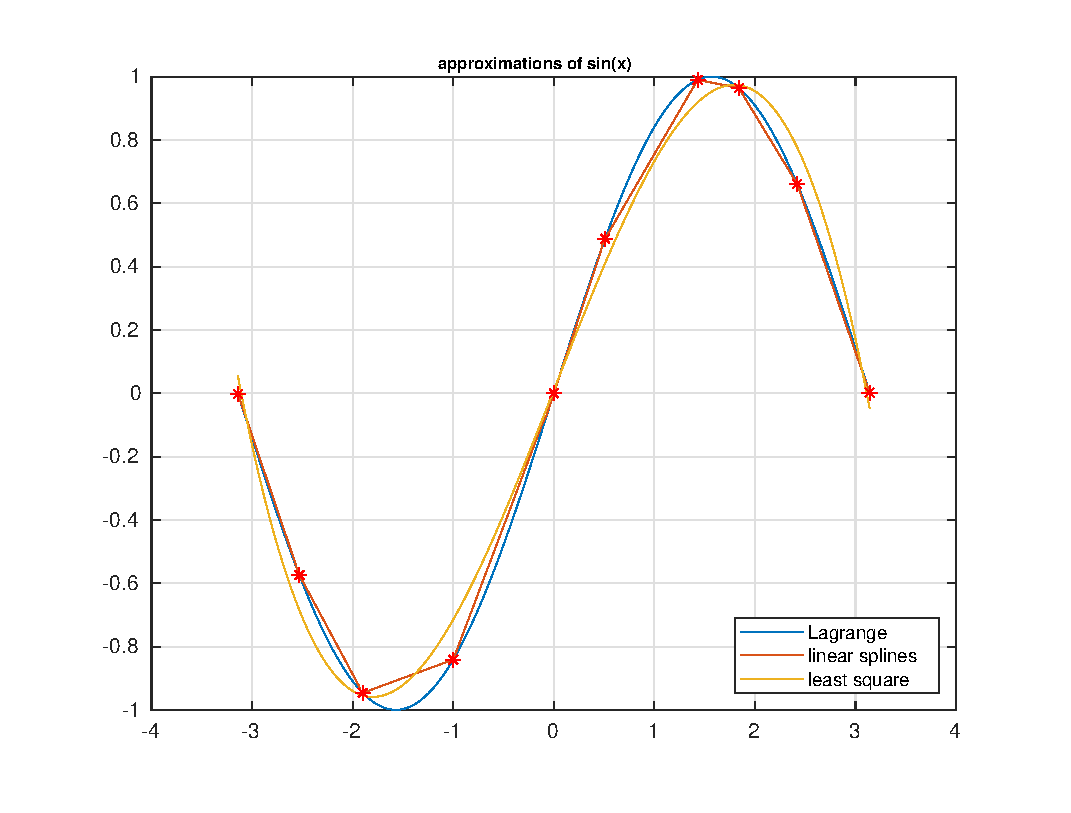
\includegraphics[width=12cm]{sinx.eps}
\end{center}
\newpage
\begin{center}
    Γραφική παράσταση του σφάλματος για κάθε τιμή της $f(x)=\mathrm{\sin\left(x\right)}$.
    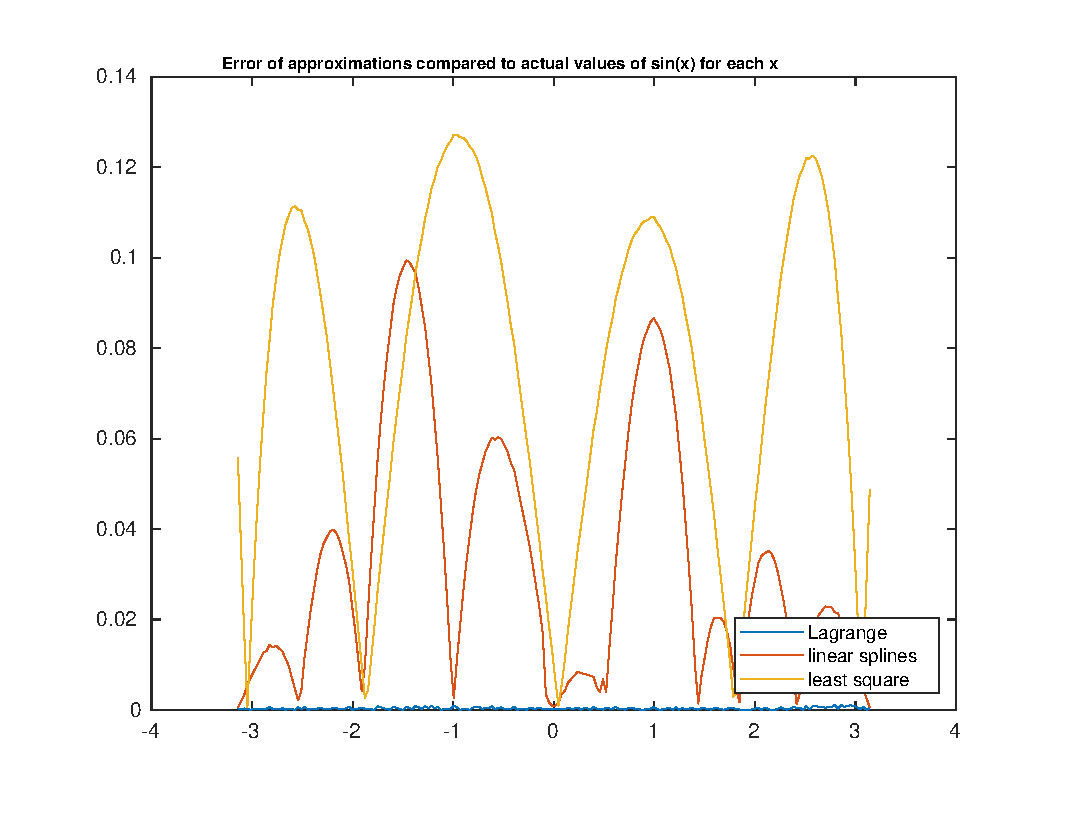
\includegraphics[width=12cm]{sinx-error.eps}\\
\end{center}
\newpage
Οι 10 τιμές $(x,y)$ που χρησιμοποιήθηκαν για την προσέγγιση της συνάρτησης είναι οι εξής:
\begin{enumerate}

    \item (-3.14,-0.002)
    \item (-2.53,-0.574)
    \item (-1.9,-0.946)
    \item (-1,	-0.841)
    \item (0,0)
    \item (0.51,0.488)
    \item (1.43,0.990)
    \item (1.84,0.964)
    \item (2.42,0.661)
    \item (3.14,0.002)
\end{enumerate}
Με την μέθοδο Lagrange η προσέγγιση του ημιτόνου στο $[-\pi,\pi]$ είναι η πιο ακριβείς όπως φαίνεται και από το διάγραμμα, με μέγιστο σφάλμα που παρατηρείται και στις 200 τιμές του $x$ να είναι ίσο με $error=0.000735$ και επιτυγχάνονται άρα 3 ψηφία ακρίβειας. \par
Για την δημιουργία μιας προσέγγισης με Splines επιλέχτηκε γραμμική spline, όπου η προσέγγιση του ημιτόνου στο $[-\pi,\pi]$ που δημιουργείται, έχει μέγιστο σφάλμα ίσο με $error=0.099119$ και πετυχαίνεται 1 ψηφίο ακρίβειας. \par
Τέλος, με την μέθοδο ελάχιστων τετραγώνων 3ου βαθμού που χρησιμοποιήθηκε, όπως φαίνεται και στο διάγραμμα η προσέγγιση δεν είναι τόσο καλή, με μέγιστο σφάλμα ίσο με $error=0.127061$ και μέση τιμή του σφάλματος να είναι ίσο με $error=0.074050$, πτωχαίνοντας έτσι οριακά ένα ψηφίο ακρίβειας στον μέσο όρο από τις 200 τιμές του $x$ στο $[-\pi,\pi]$.


\newpage 
\section{Έκτη Άσκηση}
Αρχικά, για τον υπολογισμό του σφάλματος προσέγγισης στην μέθοδο τραπεζίου θεωρητικά, χρησιμοποιείται ο 
τύπος $|e| \leq \frac{(b-a)^3}{(12\cdot N^3)}\cdot M$, 
όπου $a=0$ ,$b=\frac{\pi}{2}$, $N=$πλήθος υποδιαστηµάτων$=10$ και 
$Μ=max\{|f''(x)|:x\in[a,b]\}=1$. Άρα $|e| \leq \frac{(\frac{\pi}{2})^3}
{12\cdot 10^3} = 0.00032298204$. Για τον υπολογισμό του σφάλματος προσέγγισης θεωρητικά για την μέθοδο \lt Simpsons \gt, χρησιμοποιείται ο 
τύπος  $|e| \leq \frac{(b-a)^5}{(180\cdot N^4)}\cdot M$, όπου $Μ=max\{|f^{(4)}(x)|:x\in[a,b]\}=1$, άρα  $|e| \leq \frac{(\frac{\pi}{2})^5}
{180\cdot 10^4} = 0.00005312841$.\par 
Έπειτα από τη σχεδίαση των μεθόδων σε κώδικα, με την μέθοδο του τραπεζίου 
υπολογίζεται εμβαδό ίσο με 0.997943 και με την μέθοδο Simpsons ίσο με 
1.000003. Το σφάλμα προσέγγισης αριθμητικά λοιπόν είναι 0.002057 για την μέθοδο 
τραπεζίου και 0.000003 για την μέθοδο \lt Simpsons \gt.

\section{Έβδομη Άσκηση}

\gt
Οι τιμές κλεισίματος με τις ημερομηνίες τους που επιλέχτηκαν από την μετοχή του ΟΠΑΠ και από το κρυπτονόμισμα \lt Dogecoin \gt για την δημιουργία της προσέγγισης είναι οι εξής:
\begin{center}
\begin{tabular}{ |c|c|c|c|c| } 
 \hline
Ημερομηνία ΟΠΑΠ & Ημερομηνία \lt Dogecoin & Tιμή \lt Dogecoin & Τιμή \gt ΟΠΑΠ\\
\hline
27/9/2022 & 1/10/2022  & 0.060627 & 12.1300\\
28/9/2022 & 2/10/2022 & 0.059288 & 12.1400\\
29/9/2022 & 3/10/2022 & 0.060384 & 12.0100\\
30/9/2022 & 4/10/2022 & 0.065962 & 12.2800\\
3/10/2022 & 5/10/2022 & 0.064735 & 12.4800\\
4/10/2022 & 6/10/2022 & 0.063444 & 12.7500\\
5/10/2022 & 7/10/2022 & 0.062409 & 12.5900\\
6/10/2022 & 8/10/2022 & 0.061678 & 12.1900\\
7/10/2022 & 9/10/2022 & 0.062156 & 12.1500\\
10/10/2022 & 10/10/2022 & 0.059513 & 12.0600\\
 \hline
\end{tabular}
\end{center}
\newpage
Όπως είναι αναμενόμενο, για τις τιμές κλεισίματος που έχουμε διαθέσιμες για την δημιουργία της προσέγγισης, όσο αυξάνεται ο βαθμός του πολυωνύμου, οιπροσεγγίσεις γίνονται πιο ακριβείς. \par
Για την προσέγγιση της τιμής κλεισίματος την ημέρα των γενεθλίων (11/10/2022) καθώς και για την προσέγγιση της τιμής 5 μέρες μετά την τελευταία μέρα που χρησιμοποιήθηκε για την δημιουργία της προσέγγισης (15/10/2022), τα αποτελέσματα της μεθόδου ελάχιστων τετραγώνων είναι τα παρακάτω για κάθε βαθμό πολυώνυμου: \\

\begin{center}
    

    \begin{tabular}{ |c|c|c| }

        \hline
        Τιμή ΟΠΑΠ 11/10/2023 & 2ου βαθμού: 11.828500 &
        3ου βαθμού: 11.458000  \\
        \hline
        4ου βαθμού: 12.377500  & Πραγματική τιμή: 12.1600  & \\
         \hline
        Τιμή \lt Dogecoin \gt 11/10/2023 &2ου βαθμού: 0.057492 &
         3ου βαθμού: 0.057382 \\
        \hline
        4ου βαθμού: 0.062783  & Πραγματική τιμή: 0.060258 & \\
         \hline
        \hline
        Τιμή ΟΠΑΠ 15/10/2023 & 2ου βαθμού: 10.499924 & 
        3ου βαθμού: 7.398606 \\
        \hline
        4ου βαθμού: 24.393281 & Πραγματική τιμή: 12.7000 & \\
         \hline
        Τιμή\lt Dogecoin \gt 15/10/2023 & 2ου βαθμού: 0.044838 &
        3ου βαθμού: 0.043918  \\
        \hline
        4ου βαθμού: 0.143754 & Πραγματική τιμή: 0.058580 & \\
         \hline
    
    \end{tabular}
   
\end{center}

Όπως παρατηρείται και από τον πίνακα, για τις μετοχές του ΟΠΑΠ στην ημέρα των γενεθλίων, το πολυώνυμο του 4ου βαθμού, είναι το κοντινότερο στην πραγματική τιμή. Από την άλλη, για το  \lt Dogecoin \gt όπου οι τιμές δεν μεταβάλλονται τόσο ραγδαία, το πολυώνυμο του 2ου βαθμού είναι το πιο κοντινό και όσο αυξάνεται ο βαθμός μειώνεται η ακρίβεια. \par 
 Για την προσέγγιση της τιμής κλεισίματος 5 ημερών μετά, και στην μετοχή του ΟΠΑΠ αλλά και στο κρυπτονόμισμα \lt Dogecoin \gt, η πιο κοντινή τιμή από τις προσεγγίσεις στην πραγματική, είναι  αυτή του μικρότερου βαθμού. Αυτό είναι αναμενόμενο, καθώς στον πραγματικό κόσμο του χρηματιστηρίου, σπάνια παρατηρούνται τόσο απότομες αυξήσεις στην τιμή κλεισίματος, άρα προτιμείται και μια πιο ομαλή καμπύλη. 

% =============================================================================== %
% ||                       HERE WE END OUR DOCUMENT                          || %
% =============================================================================== %
\end{document}
